%%%%%%%%%%%%%%%%%%%%%%%%%%%%%%%%%%%%%%%%%%%%%%%%
% E.Pinault-Bigeard - e.pinault-bigeard@upsti.fr
% http://s2i.pinault-bigeard.com
% CC BY-NC-SA 2.0 FR - http://creativecommons.org/licenses/by-nc-sa/2.0/fr/
%%%%%%%%%%%%%%%%%%%%%%%%%%%%%%%%%%%%%%%%%%%%%%%%
\documentclass[11pt]{article}
%%%%%%%%%%%%%%%%%%%%%%%%%%%%%%%%%%%%%%%%%%%%%%%%
% Package UPSTI_Document
%%%%%%%%%%%%%%%%%%%%%%%%%%%%%%%%%%%%%%%%%%%%%%%%

\usepackage{import}
%
%%%%%%%%%%%%%%%%%%%%%%%%%%%%%%%%%%%%%%%%%%%%%%%%
% Package UPSTI_Document
%%%%%%%%%%%%%%%%%%%%%%%%%%%%%%%%%%%%%%%%%%%%%%%%
\usepackage{subcaption}
\usepackage[usenames, svgnames, dvipsnames]{xcolor}
\usepackage{UPSTI_Document}
\usepackage{pgfplots}
\usepackage{import}
\definecolor{darkspringgreen}{rgb}{0.09, 0.45, 0.27}

\newcommandx*{\dessinRepereFigGeo}[5][1=\vx{},2=\vy{},3=\vz{},4=,5=0]
	{
		\draw [->,very thick] (0,0) -- (1,0) ;
		\draw [->,very thick] (0,0) -- (0,1) ;
    \fill[white] (0,0) circle (0.13);
    \draw [->,very thick] (0,0) circle (0.13);
    \ifnumequal{#5}{0} {% z vers nous
      \fill[black] (0,0) circle (0.03);
      \draw [->,thick] (0,0) circle (0.04);
    }{% z vers la feuille
  		\begin{scope} [rotate=45]
  			\draw [-,thick] (0,-0.12) -- (0,0.12) ;
  			\draw [-,thick] (-0.12,0) -- (0.12,0) ;
  		\end{scope}
    }
		\draw [anchor=north west] (1.1,0) node {${#1}$};
		\draw [anchor=south west] (0,1.1) node {${#2}$};
		\draw [anchor=north east] (-0.1,0) node {${#3}$};
		\draw [anchor=north west] (-0.1,-0.1) node {${#4}$};
	}

	\usepackage{array}
	\newcolumntype{L}[1]{>{\raggedright\let\newline\\\arraybackslash\hspace{0pt}}m{#1}}
	\newcolumntype{C}[1]{>{\centering\let\newline\\\arraybackslash\hspace{0pt}}m{#1}}
	\newcolumntype{R}[1]{>{\raggedleft\let\newline\\\arraybackslash\hspace{0pt}}m{#1}}

	\usepackage{pifont}% http://ctan.org/pkg/pifont
\newcommand{\cmark}{\color{green}\ding{51}}%
\newcommand{\xmark}{\color{red}\ding{55}}%
\newcommand{\fmark}{\ding{229}}%
\newcommand{\itemc}{\item[\cmark]}%
\newcommand{\itemx}{\item[\xmark]}%
\newcommand{\itemf}{\item[\fmark]}%

\usepackage{tikz-timing}
\usepackage{circuitikz}
%---------------------------------%
% Paramètres du package
%---------------------------------%

% Version du document (pour la compilation)
% 1: Document prof
% 2: Document élève
% 3: Document à publier
\newcommand{\UPSTIidVersionDocument}{2}

% Classe
% 1: PTSI				6: PSI*			11: TSI2		16: Spé
% 2: PT	(par défaut)	7: MPSI			12: ATS
% 3: PT*				8: MP			13: PC
% 4: PCSI				9: MP*			14: PC*
% 5: PSI				10: TSI1		15: Sup
%\newcommand{\UPSTIidClasse}{2}



% Matière
% 1: S2I (par défaut)    2: IPT     3: TIPE
% 6: Vie au lycée
\newcommand{\UPSTIvariante}{5}
\newcommand{\UPSTIidMatiere}{0}
\newcommand{\UPSTIintituleMatiere}{Automatique}
\newcommand{\UPSTIsigleMatiere}{Autom}
% Type de document
% 0: Custom*				7: Fiche Métho de			14: Document Réponses
% 1: Cours (par défaut)		8: Fiche Synthèse    		15: Programme de colle
% 2: TD     				9: Formulaire
% 3: TP						10: Memo
% 4: Colle					11: Dossier Technique
% 5: DS						12: Dossier Ressource
% 6: DM						13: Concours Blanc
% * Si on met la valeur 0, il faut décommenter la ligne suivante:
%\newcommand{\UPSTItypeDocument}{Custom}
\newcommand{\UPSTIidTypeDocument}{1}

% Titre dans l'en-tête


% Titre dans l'en-tête

\newcommand{\UPSTIvariante}{5}

\newcommand{\UPSTItitreEnTete}{Automatisme industriel}
%\newcommand{\UPSTItitreEnTetePages}{}
\newcommand{\UPSTIsousTitreEnTete}{Introduction aux API}


% Titre
%\newcommand{\UPSTItitrePreambule}{Automatisme industriel}
\newcommand{\UPSTItitre}{La programmation d'un Automate Industriel}

% Durée de l'activité (pour DS, DM et TP)
\newcommand{\UPSTIduree}{3h30}

% Note de bas de première page
%\newcommand{\UPSTInoteBasDePremierePage}{Geoffrey Vaquette}
% Numéro (ajoute " n°1" après DS ou DM)
\newcommand{\UPSTInumero}{2}

% Numéro chapitre
%\newcommand{\UPSTInumeroChapitre}{1}

% En-tête customisé
%\newcommand{\UPSTIenTetePrincipalCustom}{UPSTIenTetePrincipalCustom}

% Message sous le titre
%\newcommand{\UPSTImessage}{Message sous le titre}


% Référence au programme
%\newcommand{\UPSTIprogramme}{\EPBComp \EPBCompP{B1-02}, \EPBCompP{B2-49}, \EPBCompS{B2-50}, \EPBCompS{B2-51}, \EPBCompP{C1-07}, \EPBCompP{C1-08}}

% Si l'auteur n'est pas l'auteur par défaut
%\renewcommand{\UPSTIauteur}{WWOOOOOOWW}

% Si le document est réalisé au nom de l'équipe
%\newcommand{\UPSTIdocumentCollegial}{1}

% Source
\newcommand{\UPSTIsource}{G. Vaquette, H. Discours}

% Version du document
\newcommand{\UPSTInumeroVersion}{2.0}

%-----------------------------------------------
\UPSTIcompileVars		% "Compile" les variables
%%%%%%%%%%%%%%%%%%%%%%%%%%%%%%%%%%%%%%%%%%%%%%%%


% Titre
%\newcommand{\UPSTItitrePreambule}{Automatisme industriel}
\newcommand{\UPSTItitre}{Introduction aux systèmes séquentiels}
\usetikzlibrary{arrows,automata,circuits.plc.ladder}

\newlength{\ladderskip}
\setlength{\ladderskip}{5\tikzcircuitssizeunit} % 5\tikzcircuitssizeunit = 35pt
\newlength{\ladderrungsep}
\setlength{\ladderrungsep}{.2\ladderskip}
\def\ladderrungend#1{\pgftransformyshift{-#1\ladderskip-\ladderrungsep}}

\ctikzset{
	logic ports=ieee,
	logic ports/scale=0.7,
}



\newcommand{\automaintienMachineEtat}[0]{
\begin{tikzpicture}[->,>=stealth',shorten >=1pt,auto,node distance=3cm,
                    semithick]
  %\tikzstyle{every state}=[fill=none,draw=none,text=white]

  \node[initial,state] (A)              {M1};
  \node[state]         (B) [right of=A] {M2};

  \path (A) edge [bend left]  node {$B_pM$} (B)
        (B) edge [bend left]  node {$B_pA$} (A);
\end{tikzpicture}
}


%%%%%%%%%%%%%%%%%%%%%%%%%%%%%%%%%%%%%%%%%%%%%%%%
% Début du document
%%%%%%%%%%%%%%%%%%%%%%%%%%%%%%%%%%%%%%%%%%%%%%%%
\begin{document}
\UPSTIbuildPage

%\UPSTIobjectif{Durant cette activité, nous allons analyser une trame pour l'envoi d'informations sur une étiquette.}

\tableofcontents
\pagebreak
\section{Les machines à état}

\subsection{Quelques rappels}
\UPSTIdefinition{
	Une machine d'état est une abstraction mathématique utilisée pour concevoir des algorithmes. Une machine d'état lit un ensemble d'entrées et passe à un état différent en fonction de ces entrées.}
Nous nous intéresserons aux machines déterministes à états finis. Cela signifie que lorsque la machine se trouve dans un état, il est possible de savoir vers quel état la machine va évoluer lorsque l'on connaît les entrées.

\subsection{L'auto maitien}
Nous proposons ici d'implémenter l'auto-maintien sous la forme d'une machine à états. 

\begin{UPSTIactivite}
	\UPSTIquestion{ Dessiner la machine à Etat d'un auto-maintien commandé par les boutons $B_pM$ (Marche) et $B_pA$ (Arrêt). }
	\begin{center}
		\UPSTIcorrection{\automaintienMachineEtat}

	\end{center}
\end{UPSTIactivite}

\subsection{Un tableau de classe}
Soit un tableau de classe équipé de deux boutons poussoirs et de deux capteurs fin de courses ($f_CH$ et $f_CB$ et qui suit le comportement suivant :

\UPSTIboiteCentrale{Cahier des charges - Tableau mobile}{
\begin{itemize}
	\item Le tableau est à l'arrêt
	\item Si le tableau n'est pas déjà en position haute, un appui sur $B_pM$ met en route le moteur en sens montée jusqu'à ce qu'il arrive en haut 
	\item Si le tableau n'est pas déjà en position basse, un appui sur $B_pD$ met en route le moteur en sens de déscente jusqu'à ce que le volet arrive au capteur
\end{itemize}
}
\pagebreak
\begin{UPSTIactivite}
	\UPSTIquestion{Dessiner la machine à état associée à ce comportement}

	\begin{UPSTIaCompleterEnv}
		\begin{tikzpicture}[->,>=stealth',shorten >=1pt,auto,node distance=3cm,
				semithick]
			%\tikzstyle{every state}=[fill=none,draw=none,text=white]

			\node[initial,state, initial where=above] (A)                    {M0};
			\node[state]         (B) [left of=A] {M1};
			\node[state]         (C) [right of=A] {M2};

			\path (A) edge [bend left]  node {$B_pM$} (B)
			edge [bend left]  node {$B_pD$} (C)
			(B) edge [bend left]  node {$f_CM$} (A)
			(C) edge [bend left]  node {$f_CD$} (A);
		\end{tikzpicture}
	\end{UPSTIaCompleterEnv}
\end{UPSTIactivite}


\section{Machine à état avec des bascules RS}
\subsection{Méthode}
Comme pour le LADDER, il est possible d'implémenter une machine à état sous la forme d'un circuit logique.
Pour cela, nous utiliserons des bascules RS afin de gérer les états.


\UPSTIaRetenir{
	\begin{UPSTIaCompleterEnv}
		Une démarche pour traduire une machine à état en circuits logiques est la suivante :
		\begin{enumerate}
			\item \textbf{Dessiner} la machine à état
			\item Insérer une bascule et un mémento pour chaque état
			\item Implémenter les transitions
			\begin{itemize}
				\item Prendre en compte l'état précédent
				\item Implémenter l'équation
				\item Désactiver l'état précédent tout en activant le suivant	
			\end{itemize}
			\item \textbf{Implémenter les sorties} associées aux états
		\end{enumerate}
		Par convention, les noms des variables par un $M$ pour correspondre aux momentos de LogoSoft.
	\end{UPSTIaCompleterEnv}
	%\vspace{1cm}
}

\paragraph{Représenter un état}

\UPSTIaRetenir{
Un état est représenté par une bascule RS en série avec un memento. 

Le passage de la transition de l'état suivant doit désactiver l'état actuel
}


\paragraph{Implémenter les transitions}

On passera d'un état au suivant si et seulement si la réceptivité de la transition est vérifiée et que l'état l'état précédent est actif.
Cela signifie qu'une porte ET sera obligatoirement insérée après chaque état pour prendre en compte ces deux paramètres.

Aussi, le passage d'une transition \textbf{doit} désactiver l'état précédent



\paragraph{Association des sorties}

On ajoute enfin, à la suite de chaque état, les sorties qui sont activés lors de l'activation de chaque état.

\begin{figure}
	\centering
	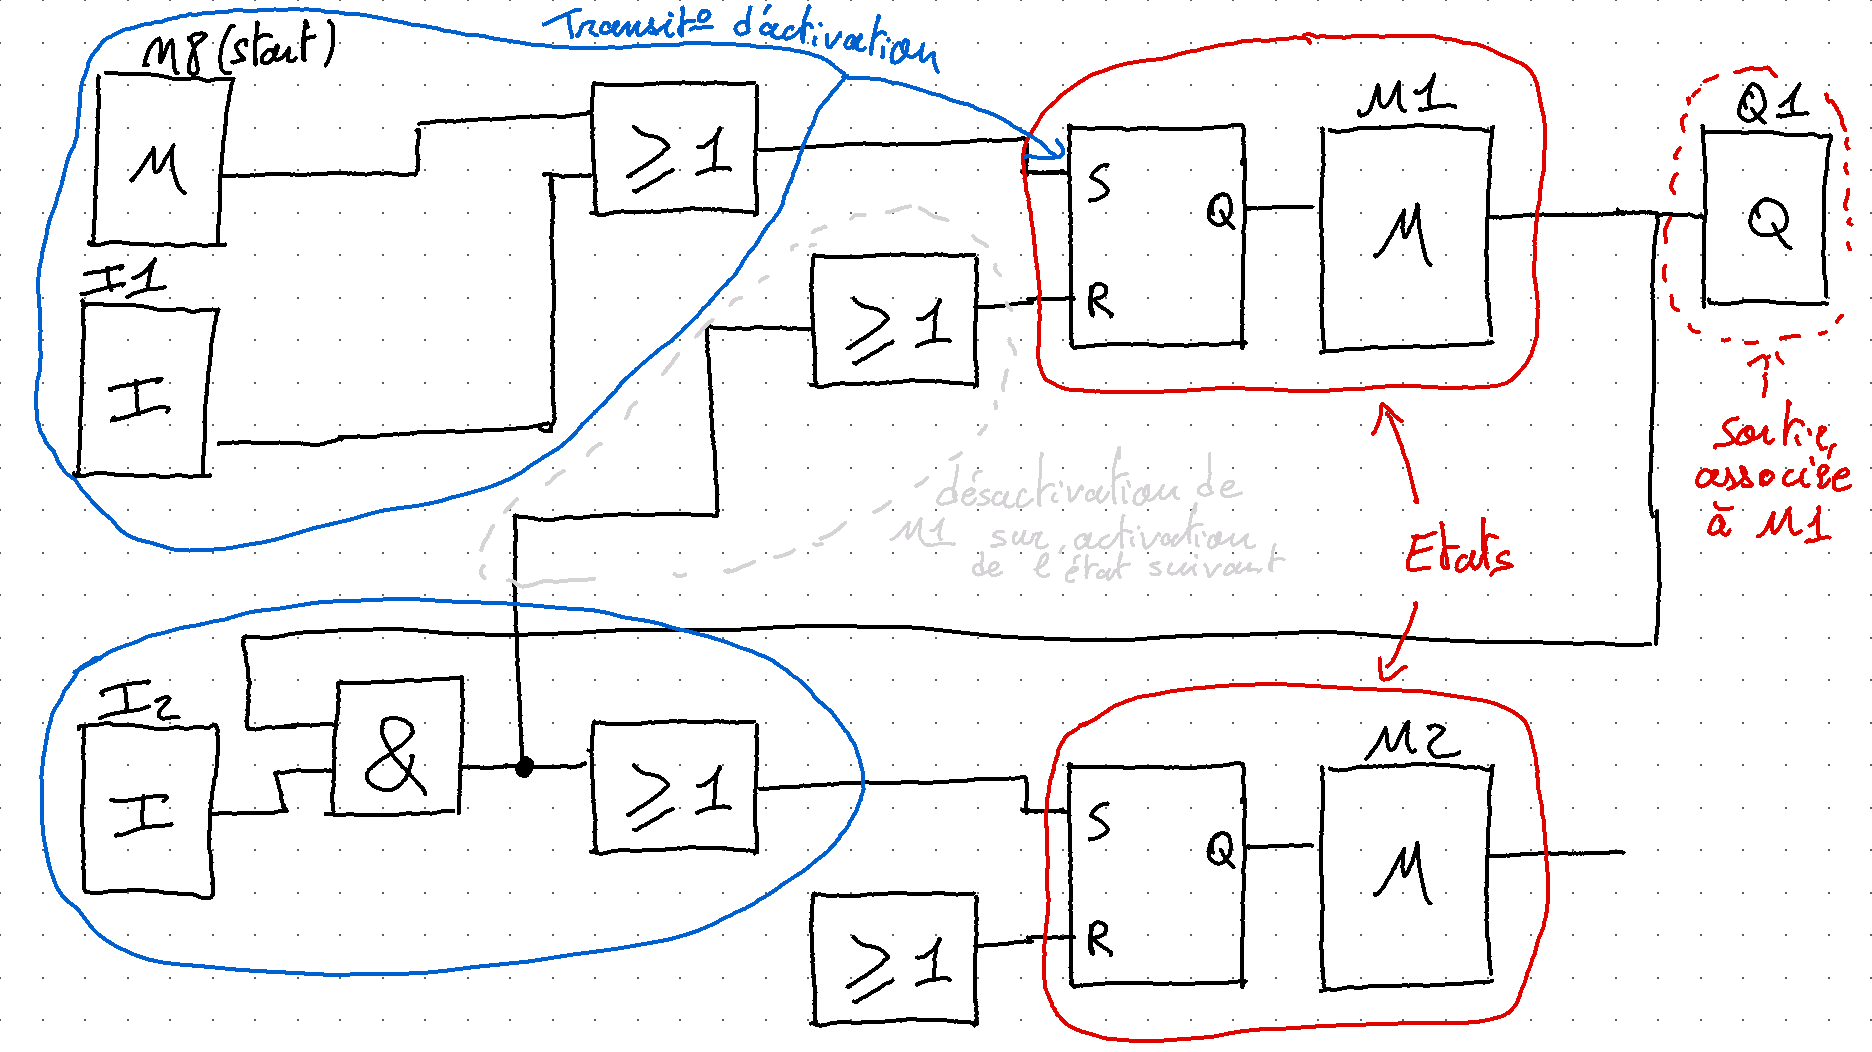
\includegraphics[width=\textwidth]{images/stateMachineToCircuit.png}
	\caption{Implémentation d'une machine à état en circuit logique}
	\label{fig:smToCircuit}
\end{figure}

\subsection{Télérupteur}
Reprenons l'exemple du télérupteur. Un télérupteur a le comportement suivant :

\UPSTIboiteCentrale{Cahier des charges - Télérupteur}{
    \begin{itemize}
        \item Au départ la lumière est éteinte
        \item Un appui sur le bouton $BP$ allume la lumière
        \item Un nouvel appui sur le bouton $BP$ éteint la lumière et on reprend à l'état initial
    \end{itemize}
}

\begin{UPSTIactivite}
	\UPSTIquestion{Dessiner la machine à état d'un télérupteur avec puis sans utilisation de front montant}

	\begin{UPSTIaCompleterEnv}

		\begin{tikzpicture}[->,>=stealth',shorten >=1pt,auto,node distance=3cm,
				semithick]
			%\tikzstyle{every state}=[fill=none,draw=none,text=white]
			\node[initial,state] (A)              {M1};
			\node[state]         (B) [right of=A] {M2};
			\path (A) edge [bend left]  node {$\uparrow B_p$} (B)
			(B) edge [bend left]  node {$\uparrow B_p$} (A);
		\end{tikzpicture}
		% \begin{tikzpicture}[->,>=stealth',shorten >=1pt,auto,node distance=3cm,
		% 		semithick]
		% 	%\tikzstyle{every state}=[fill=none,draw=none,text=white]

		% 	\node[initial,state] (A)              {0 : Arrêt};
		% 	\node[state]         (B) [right of=A] {1 : Marche};
		% 	\node[state]         (C) [right of=B] {2 : Marche};
		% 	\node[state]         (D) [right of=C] {3 : Arrêt};

		% 	\path (A) edge [bend left]  node {$B_p$} (B)
		% 	(B) edge [bend left]  node {$\overline{B_p}$} (C)
		% 	(C) edge [bend left]  node {${B_p}$} (D)
		% 	(D) edge [bend left]  node {$\overline{B_p}$} (A);
		% \end{tikzpicture}
	\end{UPSTIaCompleterEnv}

    \UPSTIquestion{En suivant le protocole, implémenter cette machine à état à l'aide d'un circuit logique.}
\end{UPSTIactivite}




\end{document}
